% ----- PLAN -----

%Computational cardiac simulations ✅
%Physical cardiac simulators and flow-loop systems
%Patient-specific cardiac and valve phantoms
%Reconstruction and modelling of valve-leaflet geometry and thickness
%Manufacturing methods and ultrasound-compatible materials
%Summary of the research gap%


\chapter{Related Work}\label{chap:related_work}
Research related to the present work spans several domains, as the development of a realistic cardiovascular phantom involves anatomical reconstruction, fluid dynamics, physical simulation, and manufacturing. From a fluid-dynamic perspective, it is necessary to first consider what can already be achieved using purely computational simulations. Such models make it possible to study cardiac motion, blood flow, and the interaction between different parts of the cardiovascular system under controlled conditions. At the same time, their results depend on assumptions and simplifications concerning the geometry, material properties, and physiological behaviour of the modelled structures \cite{BAILLARGEON201438,SUGIURA2012380,FEDELE2023115983}.

In contrast, physical cardiovascular simulators and phantoms provide an experimental environment in which blood flow, imaging methods, and medical devices can be examined directly. This raises the question of which advantages a physical reconstruction offers compared with a purely computational model and how such a reconstruction can be adapted to the anatomy of an individual patient. Patient-specific models require suitable methods for extracting anatomical information from medical image data and converting it into a manufacturable geometry. Several approaches for producing such prototypes have already been presented, including additive manufacturing and mould-based fabrication techniques \cite{sobbi2024development,engelhardt2019flexible}. 

This chapter therefore reviews computational cardiac simulations, physical cardiovascular simulators, patient-specific phantoms, and the manufacturing methods used to produce them. Particular attention is given to approaches relevant to the reconstruction and fabrication of anatomically accurate heart-valve structures.

\section{Computational Cardiovascular System Simulation}\label{sec:related_work_computational}
Using computational models to simulate the cardiovascular system can be used to study how the heart performs under healthy as well as diseased conditions. The benefit of adapting these methods instead of reverting to experiments involving patients or animals is for one the ethical aspect of completely eliminating the need for living subjects but also, when not relying on artificial physical replicas, a way to study the cardiovascular system in a highly controllable and reproducible environment. The level of detail can hereby vary widely. While some models shift their attention to the subcellular level, others describe the movement of the ventricles, the flow of blood, or even the behaviour of the entire heart. Combining these different levels is challenging because the electrical activation of the heart, the contraction of the muscles, and the resulting blood flow all influence each other. The \emph{University of Tokyo heart simulator} is an example of an approach that combines several of these processes within one computational framework. It connects models of electrical activity, muscle contraction, cardiac deformation, and blood flow. This allows the relationship between processes at the cellular level and the resulting behaviour of the heart to be investigated. However, adding more physiological detail also increases the computational effort and introduces more parameters that must be estimated or validated using experimental or clinical data \cite{SUGIURA2012380}.

Earlier computational studies frequently focused on individual parts of the heart, particularly the ventricles. More recent research has moved toward models that represent all four chambers and their interaction during the cardiac cycle. One example is the \emph{Living Heart Project}, which introduced an image-based model containing both atria and both ventricles. The model combines the electrical activation of the cardiac tissue with the resulting mechanical contraction of the heart. It can reproduce quantities such as cardiac deformation and pressure-volume relationships, which can be compared with clinical measurements. The project demonstrates how a whole-heart simulation can be used to study the combined behaviour of the different chambers rather than examining each chamber separately \cite{BAILLARGEON201438}.

Fedele et al.\ presented a more recent whole-heart model that includes additional physiological detail. Their approach considers the active contraction of both the atria and the ventricles, the orientation of the muscle fibres, differences between cardiac regions, and the connection between the heart and the circulatory system. The model reproduces several important characteristics of a healthy cardiac cycle, including changes in chamber pressure and volume, blood flow between the chambers, and the three-dimensional movement of the heart. The study also shows that atrial contraction can have an important influence on ventricular filling and should not always be neglected. Together, these projects demonstrate the continuing development of computational models toward more complete representations of cardiac function \cite{FEDELE2023115983}. But despite their increasing level of detail, the two whole-heart models discussed represent the cardiac valves in simplified forms. In the \emph{Living Heart Project}, the valves are mainly represented through their effect on the flow of blood between the chambers rather than as individual deformable leaflet structures \cite{BAILLARGEON201438}. Fedele et al.\ include the valves as simplified geometric regions within the openings between the cardiac chambers and vessels \cite{FEDELE2023115983}. These simplifications are appropriate because both projects focus mainly on the overall electrical and mechanical behaviour of the heart. However, the models do not reproduce details such as the patient-specific shape, local deformation, or spatially varying thickness of individual valve leaflets.

Therefore computational models are useful for studying the interaction between electrical activation, cardiac contraction, and blood flow. They can also be used to compare different physiological conditions and investigate processes that are difficult to observe directly. Nevertheless, their results depend on the assumptions, input data, and parameter values used to construct the model. In addition, a computational model cannot replace every type of physical experiment. Physical cardiac simulators and phantoms provide a complementary approach by creating a tangible model that can be used for experimental measurements and medical-device testing \cite{lee2026ventricular}. This makes physical phantoms particularly relevant when the geometry and physical properties of a specific anatomical structure, such as the mitral valve of a single patient, is the main subject of investigation. 

\section{Physical Cardiovascular Simulators and Phantoms}\label{sec:related_work_physical}
While the strengths of computational \emph{in silico} models lie in their ability to simulate cardiac behaviour reliably and reproducibly and to support clinical observations, the physical approach is motivated by several particularly interesting factors. Applications range from producing realistic replicas for teaching and training, to demonstrating operative procedures and treatments to patients and involving them in these processes, to presurgical planning and medical device testing, and even to printing implants for use in patient surgery. The latter has gained considerable traction in recent years and could offer substantial benefits if refined and widely adopted; this will be discussed further in Chapter~\ref{chap:conclusion} \cite{tuncay20193d}. The major distinction from computational models it that many measurements and obsercations can be made as well - although the behaviour can be reproduced only experimentally - plus the additional benefits of possessing a tangible model which can be used for several other purposes as mentioned above \cite{lee2026ventricular}.

\subsection{Source Data Acquisition and Preprocessing}\label{subsec:data_acquisition_preprocessing}
In a 2019 review, a PubMed search was conducted to assess the state of the art in 3D-printed cardiac valve models. The authors searched for English-language publications indexed up to January 2018 using the terms \emph{3D printing} AND \emph{cardiac valve}, yielding 64 results. After screening for relevance and adding papers from reference lists, 29 publications remained \cite{tuncay20193d}. The same search in September 2026 yielded 262 results. This is an unfiltered count, however, and the number of relevant publications is likely lower. Between February 2018 and September 2026, 185 items were added to the search results, suggesting a substantial increase in publications matching these terms. Many of these studies required medical imaging data for model reconstruction, making it important to consider how these data are acquired and processed.

The creation of a patient-specific physical phantom begins with the acquisition of medical image data. The choice of imaging modality determines which anatomical structures can be visualised and modelled, as well as the additional processing steps required to produce a manufacturable model. A systematic review published in 2026 analysed 63 studies on three-dimensional printing in mitral valve disease. Computed tomography (\emph{CT}) was the most commonly reported modality, used in 22 studies. Transoesophageal echocardiography (\emph{TEE}), a form of ultrasound imaging and the modality used for the data of this thesis, was reported in 16 studies. CT and TEE were used together in 10 studies, while magnetic resonance imaging (\emph{MRI}) was reported in only three \cite{pavlykova20263d}. 

\subsubsection{Computed Tomography}\label{subsubsec:computed_tomography}
The suitability of an imaging dataset for model production depends on sufficient spatial resolution, clear tissue contrast, and minimal artifacts and noise. Motion during CT acquisition can affect image quality, but cardiac and respiratory motion can be addressed through \emph{ECG gating}, \emph{breath-hold} techniques, and/or \emph{respiratory gating} in combination with a high-resolution scan \cite{tuncay20193d}. ECG and respiratory gating synchronise image acquisition with the cardiac and respiratory cycles, respectively, helping to reduce motion artifacts. Breath-hold techniques require the patient to hold their breath during the scan and can also reduce respiratory motion artifacts \cite{giraud2013respiratory}. 

In general, CT imaging fulfils the requirements for producing a physical cardiovascular phantom, as it provides high spatial resolution and sufficient contrast for the segmentation of many cardiac structures. ECG-gated multiphase acquisitions can additionally be used to reconstruct the anatomy at a selected phase of the cardiac cycle \cite{tuncay20193d}. CT is particularly suitable for obtaining accurate measurements of cardiac structures and for visualising calcifications. However, it involves exposure to ionising radiation, may require the administration of a contrast agent, and provides limited information about the tissue composition of the valve and myocardium \cite{tuncay20193d,zheng2021application}.

\subsubsection{Ultrasound}\label{subsubsec:ultrasound}
Echocardiography is commonly used as the first-line imaging modality for the assessment of heart-valve disease. It is widely available and compared to the others it provides real-time information about valve morphology, leaflet motion, blood flow, and haemodynamic function. Transthoracic echocardiography (\emph{TTE}) is non-invasive and comparatively simple to perform, whereas transoesophageal echocardiography (\emph{TEE}) can provide more detailed images of the valve and surrounding structures. In particular, three-dimensional transoesophageal echocardiography can capture the spatial geometry and motion of the valve apparatus. However, TEE is a semi-invasive procedure that commonly requires sedation and may be unsuitable for patients with certain oesophageal conditions \cite{zheng2021application}.

For the production of a patient-specific model, a three-dimensional ultrasound acquisition is required to obtain a volumetric dataset from which the anatomical structures can be segmented. The resulting image quality can nevertheless depend on the available acoustic window and the acquisition settings. Acoustic shadowing, image artifacts, and limited visibility of thin structures may make the boundaries of the valve leaflets difficult to identify. Consequently, the quality of an ultrasound-derived phantom depends strongly on the quality of the acquired volume and the reliability of the subsequent segmentation \cite{tuncay20193d,zheng2021application}. 

\begin{figure}[ht]
  \centering
  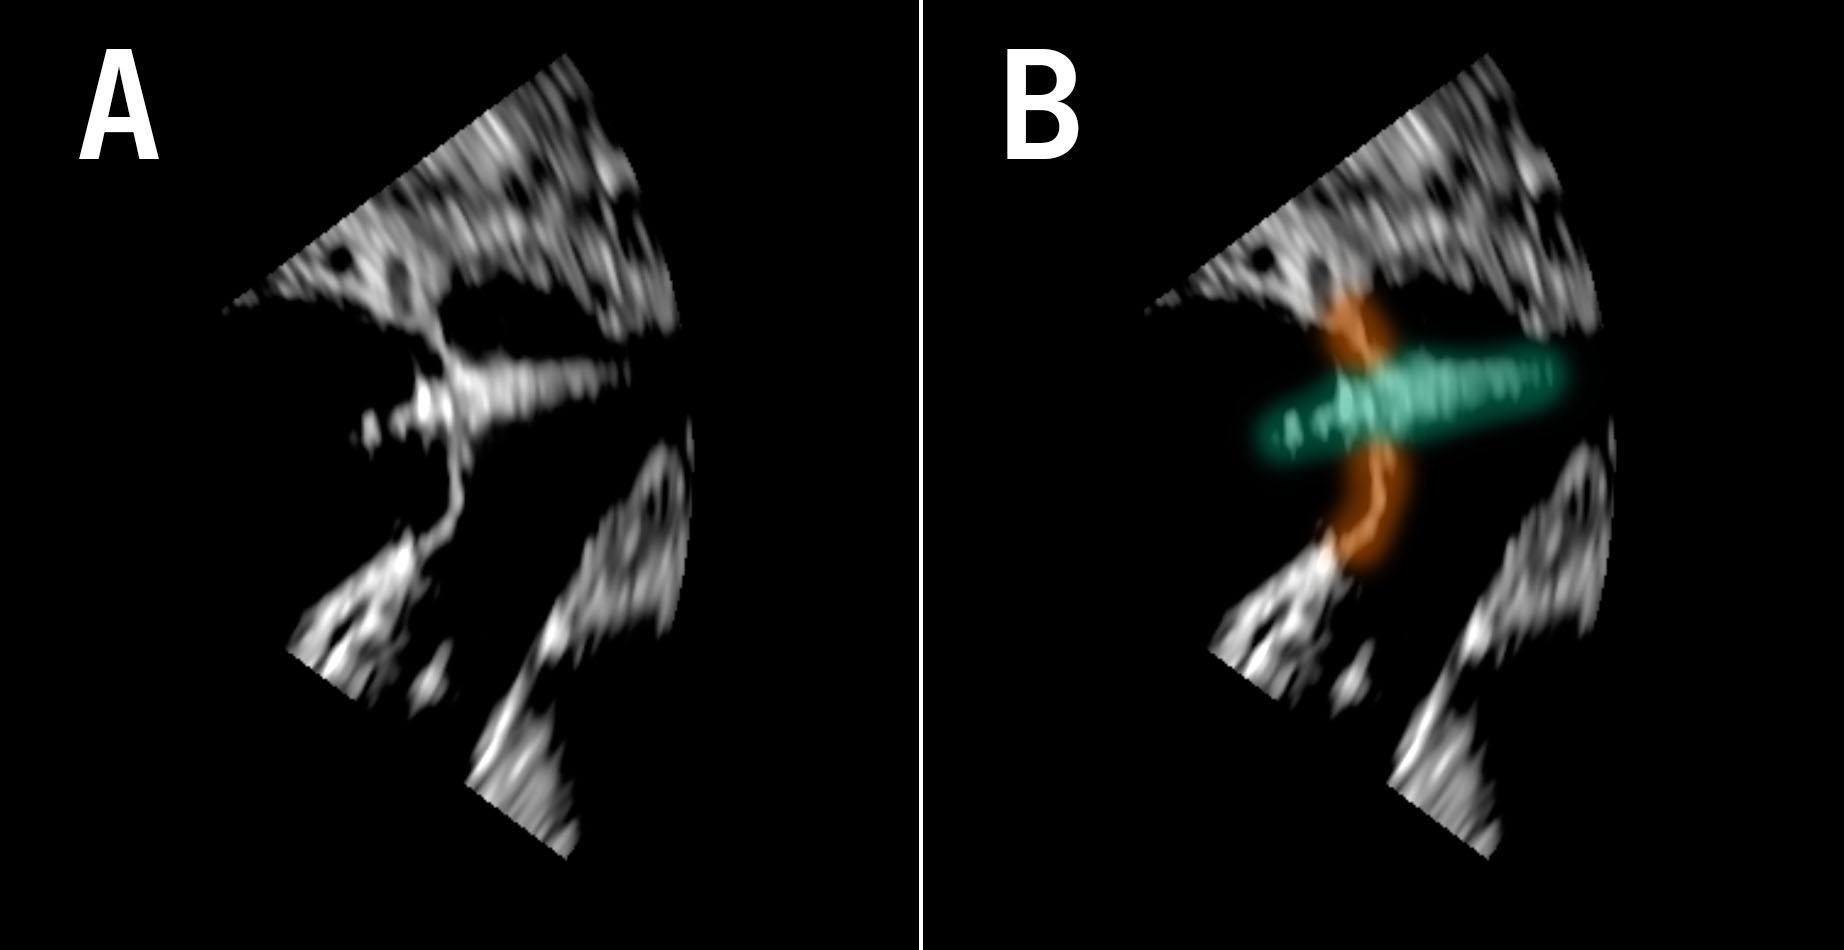
\includegraphics[width=0.75\linewidth]{graphics/coronal_view_of_ultrasound_data.jpg}
  \caption{(A) Original ultrasound image. (B) Color-coded image with visible sections of the mitral valve highlighted in orange and probe-related ultrasound artifacts highlighted in green. \textit{The colors were selected to remain distinguishable to readers with color-vision deficiencies.}}
  \label{fig:coronal_ultrasound}
\end{figure}

To provide an example Figure~\ref{fig:coronal_ultrasound} shows a coronal slice of the ultrasound data used to derive the model presented in this thesis, specifically the thickness measurements of the mitral valve leaflets, which are discussed further in Section~\ref{sec:measure}. The figure also illustrates the challenge of reliably identifying and segmenting the leaflets in the presence of ultrasound artifacts and noise. \emph{Image A} (right) shows the original, unaltered ultrasound image, while \emph{Image B} (left) has been color-coded to highlight the visible portions of the mitral valve leaflets in orange and ultrasound artifacts associated with the TEE probe in green. The colored overlays are provided for visualisation only and do not represent a segmentation.

\subsubsection{Magnetic Resonance Imaging}\label{subsubsec:ultrasound}



